\documentclass{beamer}
% \mode<presentation>{}

\usepackage[utf8]{inputenc}
\usepackage[english]{babel}
\usepackage[backend=biber,style=ieee]{biblatex}
\usepackage{colortbl}
\usepackage{graphicx}

\usetheme{AnnArbor}

\beamertemplatenavigationsymbolsempty

\setbeamertemplate{footline}[frame number]

\graphicspath{{.img/}}

\addbibresource{references.bib}

\definecolor{sea}{RGB}{175,255,215}

\begin{document}

\title{Seed-based Functional Connectivity Analysis of Hippocampal
Network of Patients Suffering from Major Depressive Disorder}

\author[]{
  \vskip -20pt
  \begin{figure}[H]
    \centering
    
\includegraphics[width=0.21\textwidth]{.img/cbeas-logo.png}
  \end{figure}
  \vskip -5pt
  College of Biomedical Engineering and Applied Sciences
}

\institute{
  \vskip -10pt
  \textit{\footnotesize Presented By:} \\[1.5mm]
  Lucky~Chaudhary~[$A27$] \and \vskip -10pt
  Namrata~Tamang~[$B3$] \and \vskip -10pt
  Nikin~Baidar~[$B4$] \and \vskip -10pt
  Nilima~Sangachchhe~[$B5$] \and \vskip -10pt
  Shashwot~Khadka~[$B18$] \and \vskip -10pt
  Sneha~Khadka~[$B22$] \and \vskip -10pt
  Suhana~Chand~[$B23$] \vskip -5pt
}

% \date{\footnotesize \vskip -20pt \hskip 205pt \today}
\date{}

\begingroup

\setbeamerfont{title}{size=\large}
\setbeamerfont{author}{size=\scriptsize}
\setbeamerfont{institute}{size=\footnotesize}

% \setbeamertemplate{headline}{}
\setbeamertemplate{footline}{}

\begin{frame}
  \vskip -5pt
  \titlepage
\end{frame}

\endgroup

\begingroup

\setbeamertemplate{footline}{}

\begin{frame}[t]
  \frametitle{Table of Contents}
  \tableofcontents
  \section{Introduction}
  \section{Major Depressive Disorder}
  \section{Brain Networks}
  \section{Functional Connectivity}
  \section{Problem Statement}
  \section{Functional MRI}
  \section{Hippocampal Network}
  \section{Objectives}
  \section{Methodology}
  \section{Feasibility of the Project}
  \section{Proposed Workflow}
  \section{Cost Estimations}
  \section{Conclusion}
  \section{References}
\end{frame}

\endgroup

\begingroup

\logo{
\includegraphics[width=0.1\textwidth]{.img/cbeas-logo.png}}
\addtocounter{framenumber}{-2}

  \begin{frame}[t]
    \frametitle{Introduction}

      \vskip 20pt

    \begin{itemize}

      \item Mental Disorders can occur when the brain or a part of the
        brain is not working well or is working in the wrong
        way. \vskip 10 pt

      \item Different type of depression exist, with symptoms ranging
        from relatively minor to severe. \vskip 10pt

      \item Major Depressive Disorder or Major Depression is a common
        and a serious mental disorder \vskip 10pt

      \item WHO claims that over 264 million people of all ages suffer
        from depression worldwide

    \end{itemize}


  \end{frame}

  \begin{frame}[t]
    \frametitle{Major Depressive Disorder}

      Depression disrupts several brain functions

      \vskip 20pt
    \begin{figure}[H]
      \centering
      % 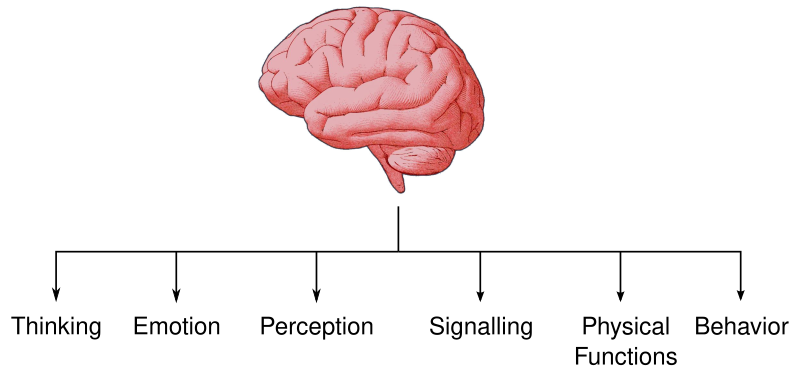
\includegraphics[width=0.8\textwidth]{brain-function-disruptions.jpg}
      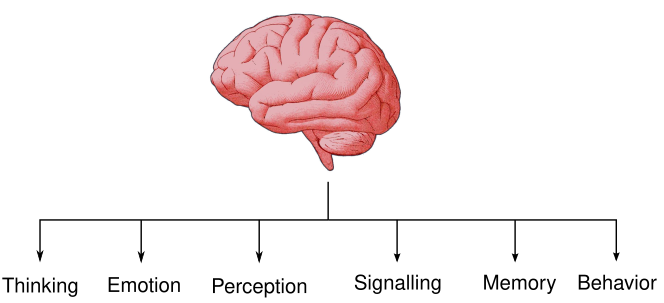
\includegraphics[width=0.8\textwidth]{mdd-brain-function-disruptions.png}
      \caption{Brain functions disrupted by MDD}
    \end{figure}

    %====================================================================%
    % Thinking - Cognition                                               %
    % Perception or sensing                                              %
    % Emotion or feeling                                                 %
    % Signalling means being responsive and reacting to the environment  %
    % Physical or somatic People's ability to perform physical tasks get %
    % disrupted                                                          %
    % Behavior                                                           %
    %====================================================================%


  \end{frame}

  \begin{frame}[t]
    \frametitle{Symptoms of MDD}

    \begin{itemize}

    \item MDD is characterized by an array of symptoms, although
      symptoms can vary from person to person \vskip 5pt

    \item MDD is diagnosed on the basis of behavioral observations and
      patient reported symptoms

    \end{itemize}

    \begin{figure}[H]
      \centering
      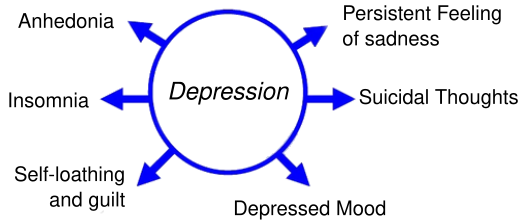
\includegraphics[width=0.7\textwidth]{depression-symptoms.png}
      \caption{Common Symptoms of MDD}
    \end{figure}

  \end{frame}

  \begin{frame}[t]
    \frametitle{Brain Networks}

    \vskip 10pt

    \begin{itemize}
      \item Collection of brain regions working together to produce
        a specific function \vskip 5pt

      \item Brain regions in a network do not have to be physically connected
        \vskip 5pt

      \item Six major large scale brain networks:
        \vskip 5pt
        \begin{enumerate}
          \item Default Mode Network
          \item Salience Network
          \item Dorsal Attention Network
          \item Frontoparietal Attention Network
          \item Sensorimotor Network
          \item Visual Network
        \end{enumerate}
        \vskip 5pt

      \item The hippocampal network is a part of the Default Mode
        Network


    \end{itemize}

  \end{frame}

  \begin{frame}[t]
    \frametitle{Diagrammatic Representation of Core Brain Networks}
    \framesubtitle{Brain Networks Continued..}

    \begin{figure}[H]
      \centering
      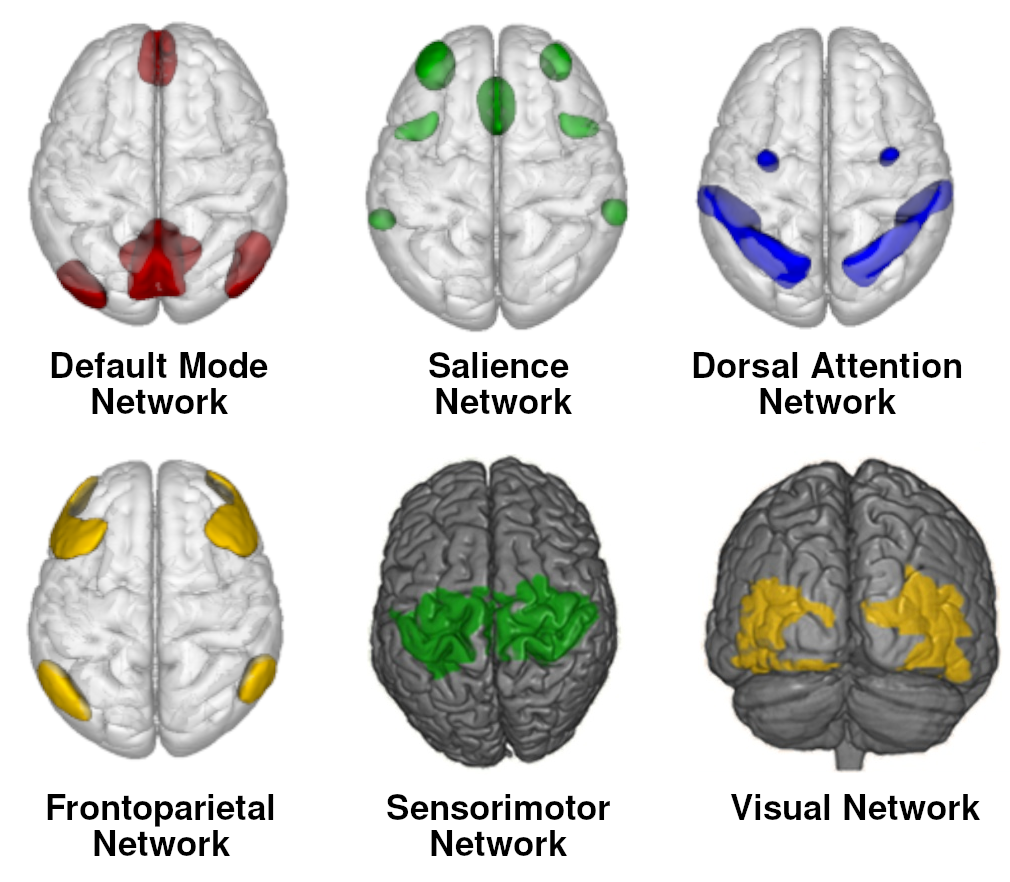
\includegraphics[width=0.6\textwidth]{brain-networks.png}
      \caption{Core Brain Networks}
    \end{figure}

  \end{frame}


  \begin{frame}[t]
    \frametitle{Functional Connectivity}

    \vskip 25pt

    \begin{itemize}
      \item Cognitive tasks are performed not by an individual brain
        region working in isolation but rather by brain networks
        consisting of several discrete brain regions that are said to
        be ``functionally connected''. \vskip 10pt

      \item Defined as temporal correlation between spatially remote
        neurophysiological events. \vskip 10pt

      \item Functional connectivity of brain networks can be
        acknowledged through statistical analysis of spontaneously
        generated BOLD signals between brain regions.

    \end{itemize}

  \end{frame}

  \begin{frame}[t]
    \frametitle{Resting State Functional Connectivity}
    \framesubtitle{Functional Connectivity Continued..}

    \vskip 20pt


    \begin{itemize}

      \item Resting state functional connectivity measures the
        temporal correlation of spontaneous BOLD signals among
        spatially distributed brain regions when the brain is not
        performing any specific task or is at rest. \vskip 10pt

      % \item Used in brain mapping to evaluate region interactions that
      %   occur in a resting or task negative state i.e. when an
      %   explicit task is not being performed. \vskip 10pt

      \item Seed-based Correlation Analysis (SCA) and Independent
        Component Analysis (ICA) are two methods that are most
        commonly used to examine resting state functional connectivity
        of brain networks. \vskip 10pt

      \item In SCA, activity is extracted from a specific region of
        interest which is then correlated with the rest of the brain.

    \end{itemize}

  \end{frame}

  \begin{frame}[t]
    \frametitle{Problem Statement}

    \begin{figure}[H]
      \centering
      \vskip 20pt
      \hskip -60pt
      
\includegraphics[width=\textwidth]{fishtail.png}
      \caption{Fishbone chart representing Problem Statement}
    \end{figure}

  \end{frame}

  \begin{frame}[t]
    \frametitle{Functional MRI (fMRI)}

    \begin{itemize}
      \item Functional neuroimaging involves imaging of brain
        functions, in contrast to structural neuroimaging which
        involves visualization of brain structures. \vskip 10pt

      \item Functional neuroimaging opts for mapping brain functions
        or depicting disease-related molecular changes that occur
        independently of structural changes. \vskip 10pt

      \item fMRI relates to blood oxygen level-dependent (BOLD)
        signal, which is generated due to a transient and local access
        of oxygenated blood, resulting from changes in regional CBF and
        neuronal activity. \vskip 10pt

      \item Captures changing blood flow in the brain which reflects
        which brain structures are activated during performance of
        different tasks.

    \end{itemize}

  \end{frame}

  \begin{frame}[t]
    \frametitle{Hippocampal Network}
    \framesubtitle{Diagrammatic Representaion of Hippocampal Circuitry}

    \vskip 10pt

    \begin{figure}[H]
      \centering
      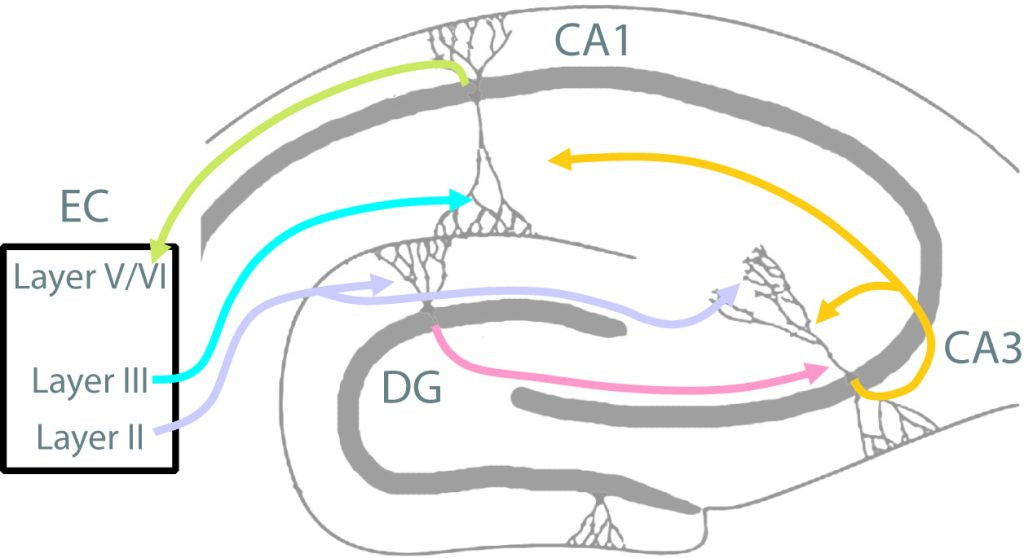
\includegraphics[width=0.7\textwidth]{hippocampal-circuitry.jpg}
      \caption{Hippocampal Circuitry}
    \end{figure}

  \end{frame}

  \begin{frame}[t]
    \frametitle{Objectives}

    \vskip 15pt

    \begin{figure}[H]
      \centering
      
\includegraphics[width=\textwidth]{objectives.png}
      \caption{Chart representing Objectives}
    \end{figure}

  \end{frame}

  \begin{frame}[t]
    \frametitle{Methodology}

    \begin{figure}[H]
      \centering
      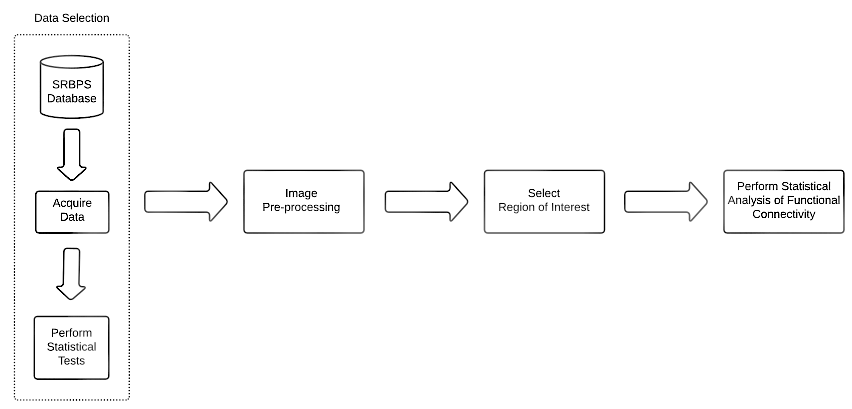
\includegraphics[width=\textwidth]{methodology-flowchart.png}
      \caption{Flowchart representing Methodology}
    \end{figure}

  \end{frame}


  \begin{frame}[t]
    \frametitle{Feasibility of the Project}

    \begin{itemize}

      \vskip 25pt

      \item  Many researches have been conducted worldwide that
        involves similar approaches for the exploration of functional
        connectivity. \vskip 10pt

      \item fMRI images will be retrieved form the DecNef Project
        Brain Data Repository. \vskip 10pt

      \item Open-source softwares such as AFNI and the Linux operating
        system will be used. \vskip 10pt

      \item The work involved in this project can be conducted
        virtually at home, therefore this eliminates the obstacles
        that may arise due to the on-going pandemic.

    \end{itemize}

  \end{frame}

  \begin{frame}[t]
    \frametitle{Proposed Workflow}

    \vskip 10pt
    \begin{figure}[H]
      \centering
      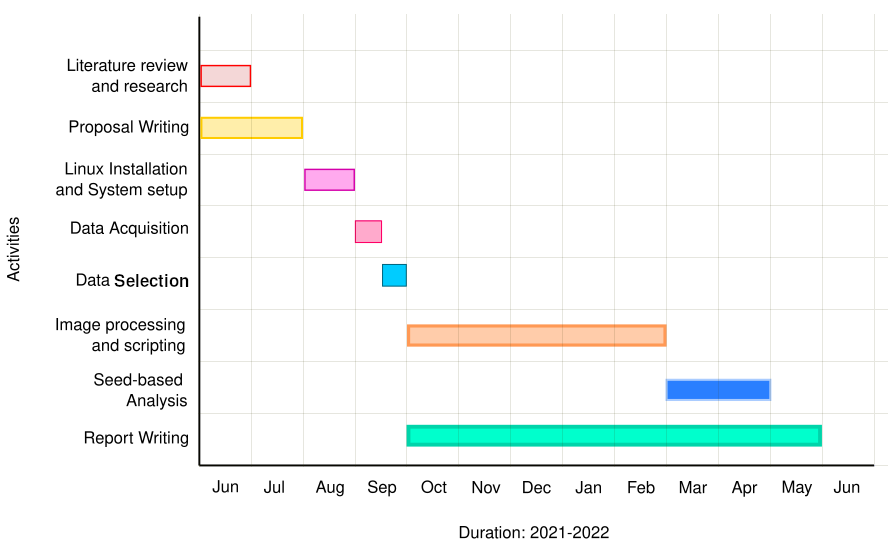
\includegraphics[width=0.8\textwidth]{proposed-workflow.png}
      \caption{Gantt Chart representing Proposed Workflow}
    \end{figure}

  \end{frame}


  \begin{frame}[t,fragile]
    \frametitle{Cost-Estimations}

    The budget plan for this project is tabulated below:
    \vskip 20pt

    \begin{table}[H]
      \newcolumntype{P}[1]{>{\centering\arraybackslash}p{#1}}
      \centering
      \begin{tabular}{|c|m{5cm}|P{1cm}|P{1cm}|P{2cm}|}
        \hline
        S.N. & \multicolumn{1}{c|}{Cost Element} & Rate
        (NRs.) & Units & Total Cost (NRs.)\\ \hline
        1 & SANDISK SATA SSD (512 GB) &  8,500 & 4 & 34,000 \\ \hline
        2 & External HDD (1 TB) &  4,000 & 1 & 4,000 \\ \hline
        3 & Miscellaneous &  - & - & 7,000 \\ \hline
          \rowcolor{sea}
        4 & \multicolumn{3}{c|}{Grand Total} &
        \multicolumn{1}{c|}{45,000} \\ \hline
      \end{tabular}
      \caption{Cost Estimations}
    \end{table}

    So, the total estimated cost of this project is
    \textit{NRs.\hspace*{2pt}45,000 only}.

  \end{frame}


  \begin{frame}[t]
    \frametitle{Conclusion}

    \vskip 20pt

    \begin{itemize}

      \item The results of the project might not be sufficient to
        provide a detailed understanding of the complex and changing
        functional connectivity of the brain for making the actual
        diagnosis of MDD through fMRI possible.

      \item It will only lay the foundations for further reasearch and
        devlopment.
    \end{itemize}

  \end{frame}

  \begin{frame}
    \frametitle{References}
    \nocite{dataset}
    \nocite{dorsalattentionfronto}
    \nocite{hippocampalcircuitry}

    \printbibliography

  \end{frame}

  \endgroup

  \setbeamertemplate{footline}{}

  \begin{frame}[noframenumbering]
    \vspace{10pt}
    \begin{center}
      \Huge \emph{Thank You!}
    \end{center}
  \end{frame}

\end{document}
